\documentclass{beamer}

\usepackage{graphicx}
%
% Choose how your presentation looks.
%
% For more themes, color themes and font themes, see:
% http://deic.uab.es/~iblanes/beamer_gallery/index_by_theme.html
%
\mode<presentation>
{
  \usetheme{Boadilla}      % or try Darmstadt, Madrid, Warsaw, ...
  \usecolortheme{default} % or try albatross, beaver, crane, ...
  \usefonttheme{default}  % or try serif, structurebold, ...
  \setbeamertemplate{navigation symbols}{}
  \setbeamertemplate{caption}[numbered]
} 

\usepackage[english]{babel}
\usepackage[utf8x]{inputenc}

% Adicionados por Luan
\usepackage{outlines}
\usepackage{ragged2e}
\usepackage{microtype}
\usepackage[none]{hyphenat}

\graphicspath{{figures/}}

\setbeamertemplate{caption}{%
\begin{beamercolorbox}[]{}
\begin{center}
\insertcaption
\end{center}
\end{beamercolorbox}%
}

\title[Coloração de Vértices]{Coloração de Vértices}
\author{Eduardo Queiroga, Luan Teylo}
%\institute{Where You're From}
\date{09 Junho de 2017}

\begin{document}
\setbeamertemplate{footline}{}
\begin{frame}
  \titlepage
\end{frame}

% Uncomment these lines for an automatically generated outline.
%\begin{frame}{Outline}
%  \tableofcontents
%\end{frame}

\section{Definição}
% * <luanteylo@gmail.com> 2017-06-04T11:17:04.521Z:
%
% ^.

\begin{frame}{Coloração de Vértices}{Definição}

\begin{itemize}
      \item Uma \textit{$k$-coloração de vértices} de $G$ é uma atribuição de $k$ cores ($1,2,\dots,k$) em $V$. A coloração é \textbf{própria} quando vértices adjacentes recebem \textbf{cores distintas}.																	
\end{itemize}

  \begin{center}
      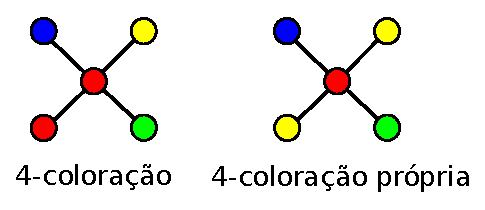
\includegraphics[scale=0.7]{color-propria.eps}
    \end{center}

  \begin{itemize}
      \onslide<2->\item Uma \textit{$k$-coloração própria} de vértices de um grafo sem \textit{loops} é um particionamento $(V_1, V_2,\dots,V_k)$ de $V$ em $k$ conjuntos independentes.
      \onslide<3->\item $G$ é dito \textit{k-colorível} se admitir uma \textit{k-coloração própria}.
  \end{itemize}
\end{frame}


\begin{frame}{Coloção de Vértices}{Definição}
    
    \begin{itemize}
        \item Claramente, um grafo é \textit{k-colorível} se e somente se o seu grafo simples subjacente for \textit{k-colorível}. Portanto, apenas grafos simples serão considerados.
    	\item Um grafo simples é \textit{1-colorível} se e somente se ele for vazio e \textit{2-colorível} se e somente se for bipartido.        
    \end{itemize}
\end{frame}




\begin{frame}{Coloração de Vértices}{Definição}

\begin{outline}
	\1 O \textbf{número cromático}  de $G$, $\chi(G)$, é o menor $k$  tal que $G$ seja $k$-colorível.
    \vskip 0.1cm
    \2 Se $\chi(G)=k$, então $G$ é dito \textit{k-cromático.}
\end{outline}

% Colocar A figura 8.1 (3-cromático)

    \begin{figure}
      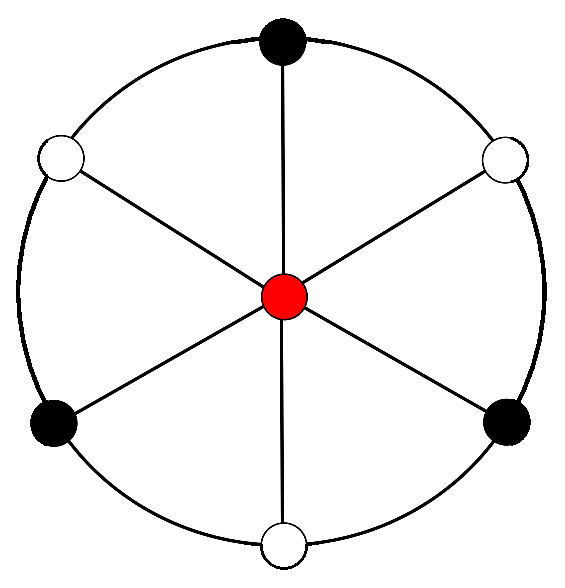
\includegraphics[scale=0.5]{3-chromatic-graph.eps}
      \caption{Grafo \textit{3-cromático}}
    \end{figure}


\end{frame}

\begin{frame}{Coloração de Vértices}{Definição}

\begin{outline}
	\1 Dizemos que um grafo $G$ é \textbf{crítico} se para todo \textit{subgrafo próprio} $H$ de $G$, $\chi(H) < \chi(G)$
	\vskip 0.2cm
	\2 Um grafo \textit{k-crítico} é aquele que é \textit{k-cromático} e crítico; todo grafo \textit{k-cromático} tem um subgrafo \textit{k-crítico}.
\end{outline}

%color A figura 8.2 (4-crítica)
    \begin{figure}
      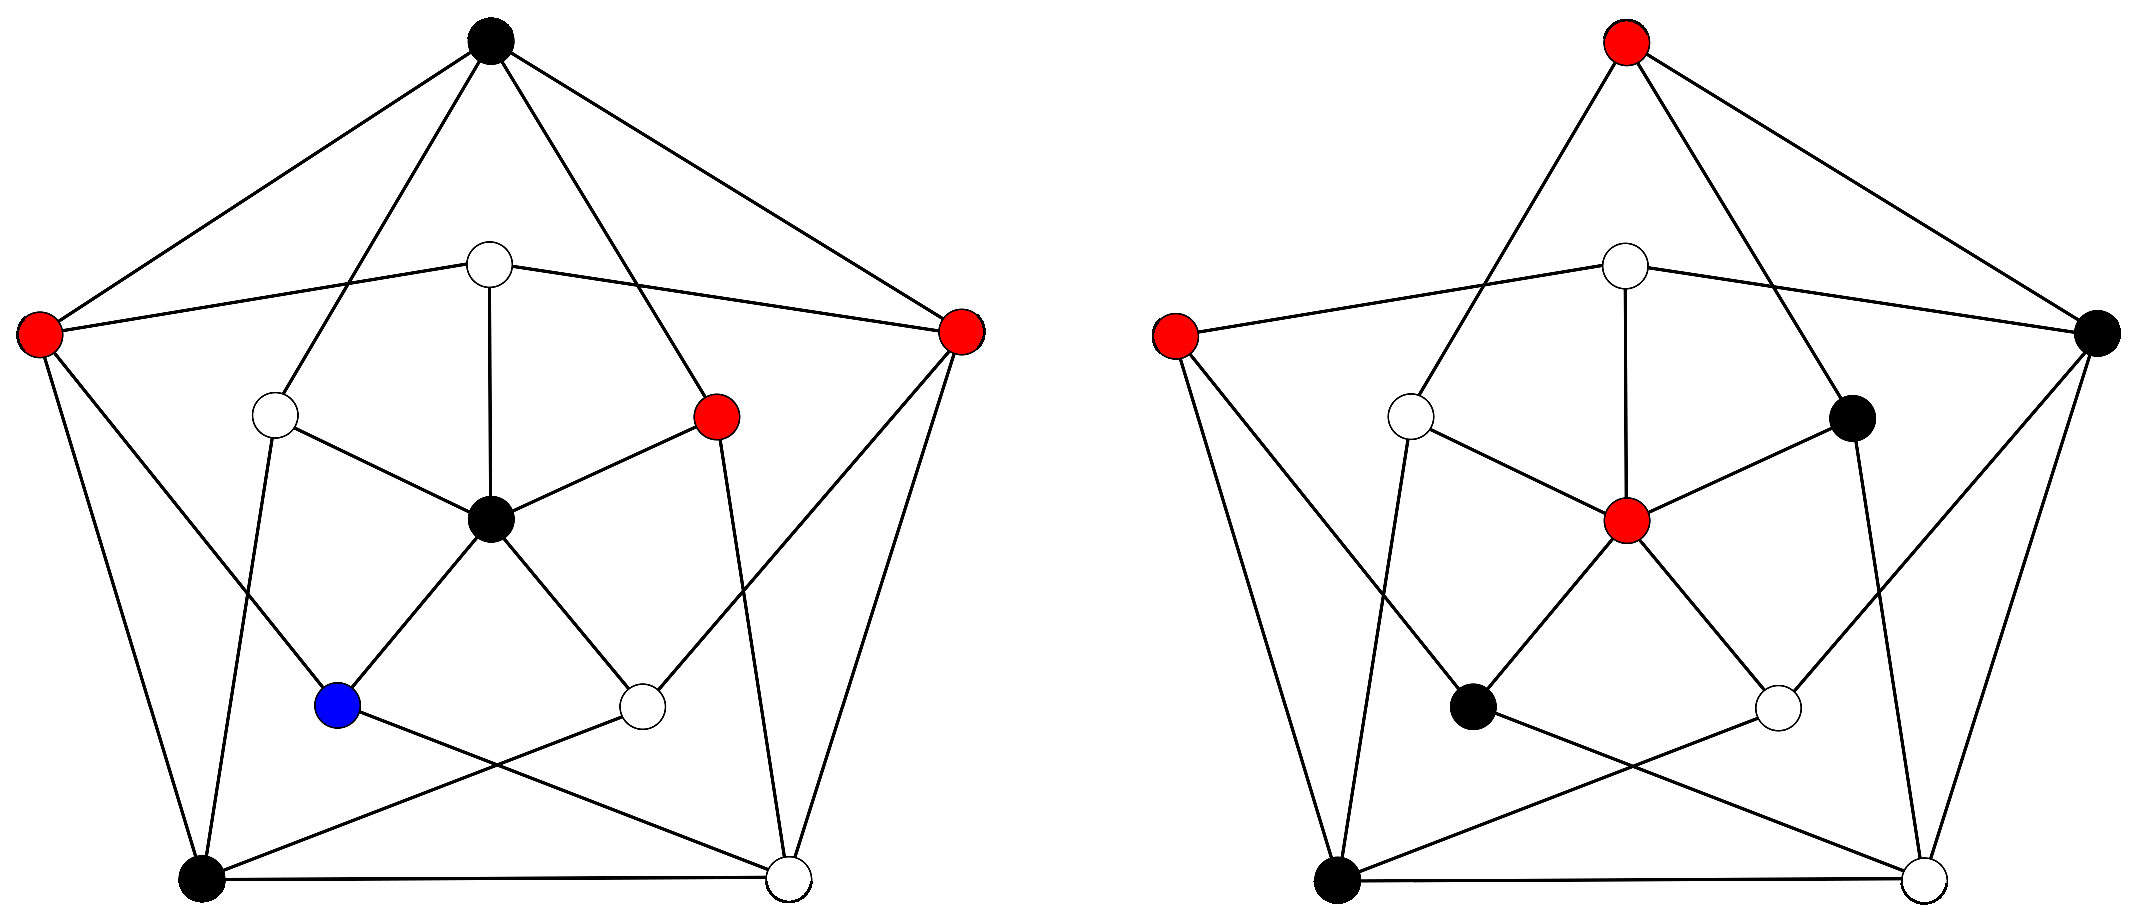
\includegraphics[scale=0.27]{grotzsch.eps}
      \caption{\textit{O grafo 4-crítico de Gr\"{o}tzsch} e um subgrafo qualquer.}
    \end{figure}
    
\end{frame}


\begin{frame}{Teorema 8.1}{}

    \only<1>{\begin{alertblock}{Teorema}
        Se $G$ é $k$-crítico, então $\delta \geq k-1$
    \end{alertblock}}
    
    
    \only{\begin{block}{Prova: }
    \begin{sloppypar}
    \justifying
    Por contradição. Se possível, seja $G$ um grafo $k$\textit{-crítico} com $\delta < k-1$, e seja $v$ um vértice de grau $\delta$ em $G$.  Uma vez que $G$ é $k$\textit{-crítico}, $G-v$ é $(k-1)$\textit{-colorível}.  
    
    \vskip 0.3cm
    
    Seja $(V_1, V_2, \dots, V_{k-1})$ uma $(k-1)$\textit{-coloração} de $G-v$.  Por definição, $v$ é adjacente em $G$ a $\delta < k-1$ vértices e, portanto, $v$ precisa ser \textbf{não adjacente} em $G$ a todo vértice de algum $V_j$.
    
    \vskip 0.3cm
    Mais então, $(V_1, V_2, \dots, V_j \cup \{v\}, \dots, V_{k-1})$ é uma $(k-1)$\textit{-coloração} de $G$. Contradição, portanto $\delta \geq k-1$.
    
    \hfill\(\square\)
    \end{sloppypar}
    \end{block}}
\end{frame}




\begin{frame}{Corolário 8.1.1}{}

\only<1>{
    \begin{alertblock}{Corolário}
        Todo grafo \textit{k-cromático} tem pelo menos $k$ vértices  com grau  $\geq k-1$
    \end{alertblock}
    
    
    
     
    \begin{figure}
      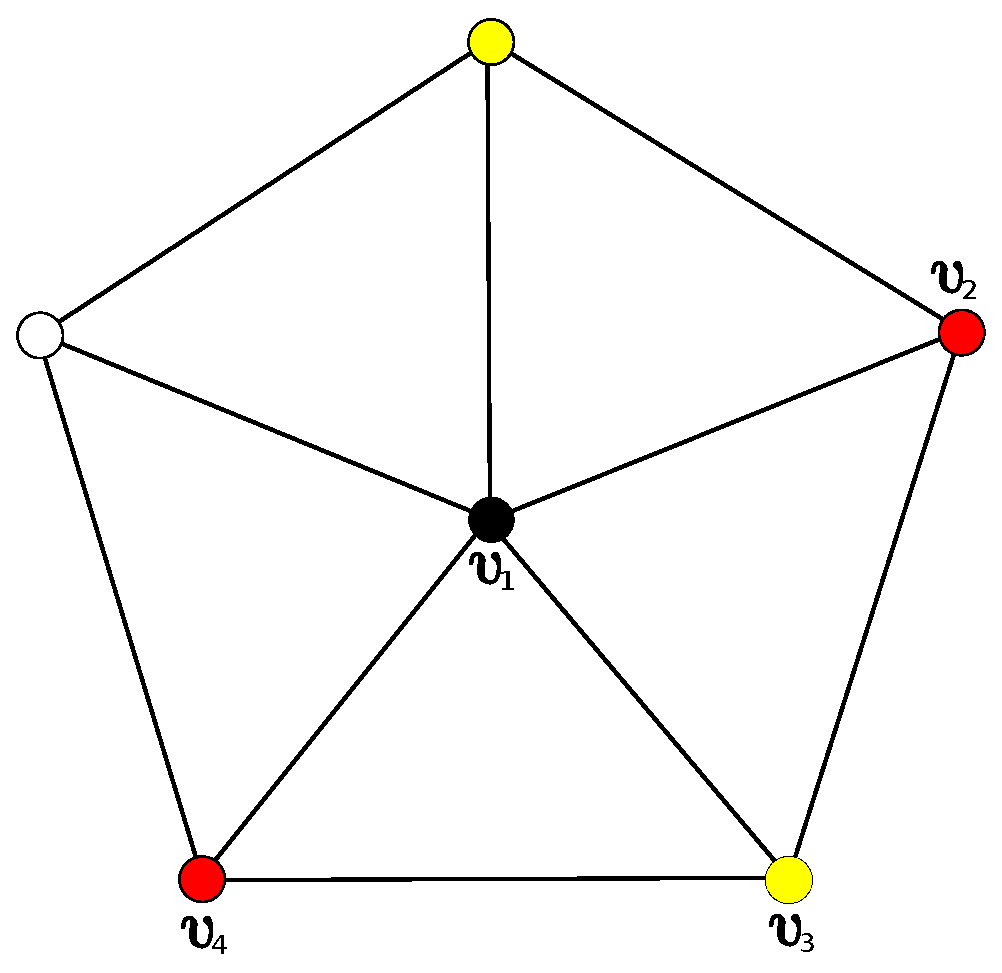
\includegraphics[scale=0.27]{4-cromatico.eps}      
      \caption{Um Grafo \textit{4-cromático}}      
    \end{figure}}
    
  
    \only<2>{
    \vskip 1cm
    \begin{block}{Prova:}
        \begin{sloppypar}
            \justifying
            Seja $G$ um grafo \textit{k-cromático}, e seja $H$ um subgrafo \textit{k-crítico} de $G$.
            \vskip 0.3cm
            Pelo teorema 8.1, todo vértice $v \in V$ têm grau de pelo menos $k-1$ em $H$ e, portanto, também em $G$. Segue então que $H$, sendo \textit{k-cromático}, claramente tem ao menos $k$ vértices.            
            
            \hfill\(\square\)
        \end{sloppypar}
    \end{block}}% fim-only<2>
\end{frame}

\begin{frame}{Corolário 8.1.2}{}
    \begin{alertblock}{Corolário}
        Para qualquer grafo $G$, $\chi \leq \Delta + 1$
    \end{alertblock}
    \vskip 1.5cm
    \begin{block}{Prova:}
        \begin{sloppypar}
            \justifying
            Suponha que a afirmação não seja verdadeira. Portanto, existe um grafo $G$ com \textit{número cromático} $\Delta + 2$.
            \vskip 0.3 cm
            Pelo teorema 8.1, deve existir pelo menos $\Delta+2$ vértices com grau maior ou igual que $\Delta +1$. Isso é impossível.            
            
            \hfill\(\square\)
        \end{sloppypar}
    \end{block}
\end{frame}


\begin{frame}{Definição}{S-Componentes}

\only<1>{
    \begin{outline}    
        \1 \justifying Seja $S$ um \textit{corte por vértice} de um grafo conexo $G$, sendo que os componentes de $G-S$ apresentam os seguintes conjuntos de vértices $V_1, V_2, \ldots, V_n$. \vskip 0.1cm
        \2 Os subgrafos $G_i = G[V_i \cup S]$ são chamados de \textbf{S-componentes} de G.
    \end{outline}
    
    %Inserir Figura 8.3
    \begin{figure}
      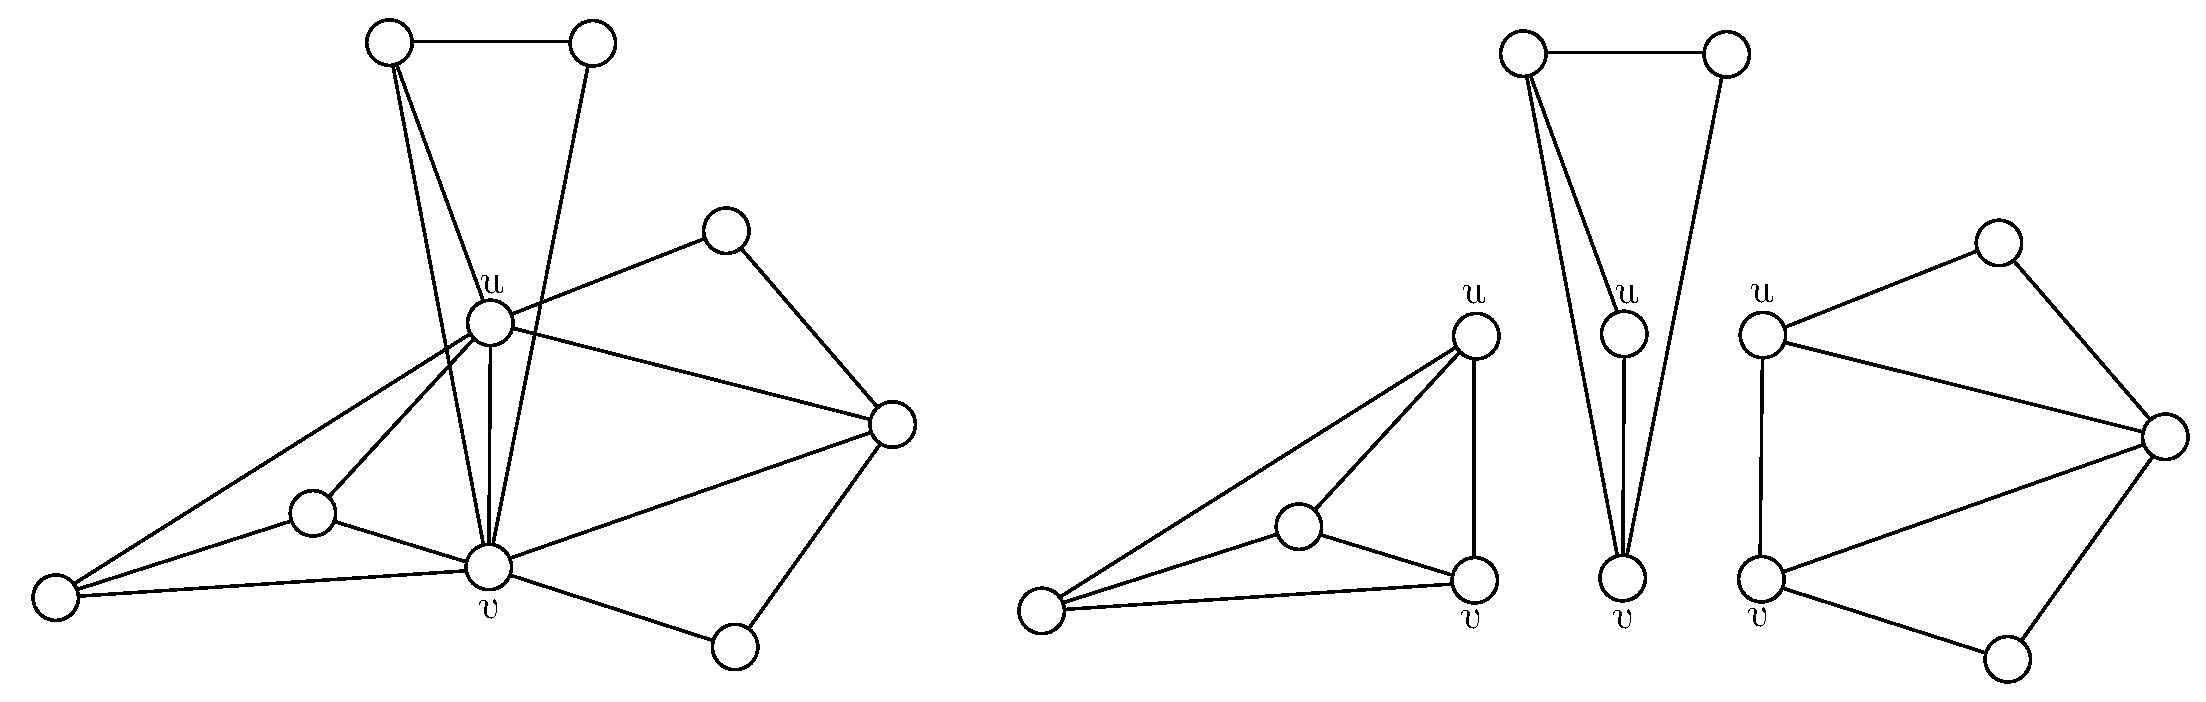
\includegraphics[scale=0.3]{s-components.eps}      
      \caption{$G$ e as suas $\{u,v\}$-componentes.}      
    \end{figure}
   
}



\only<2>{
\begin{outline}
    \1 Dizemos que as colorações de $G_1, G_2, \ldots, G_n$ \textbf{concordam} em S, se e somente se $\forall v \in S$ a atribuição de cores for igual em qualquer uma das colorações. 
\end{outline}
        %Inserir Figura Agree
    \begin{figure}
      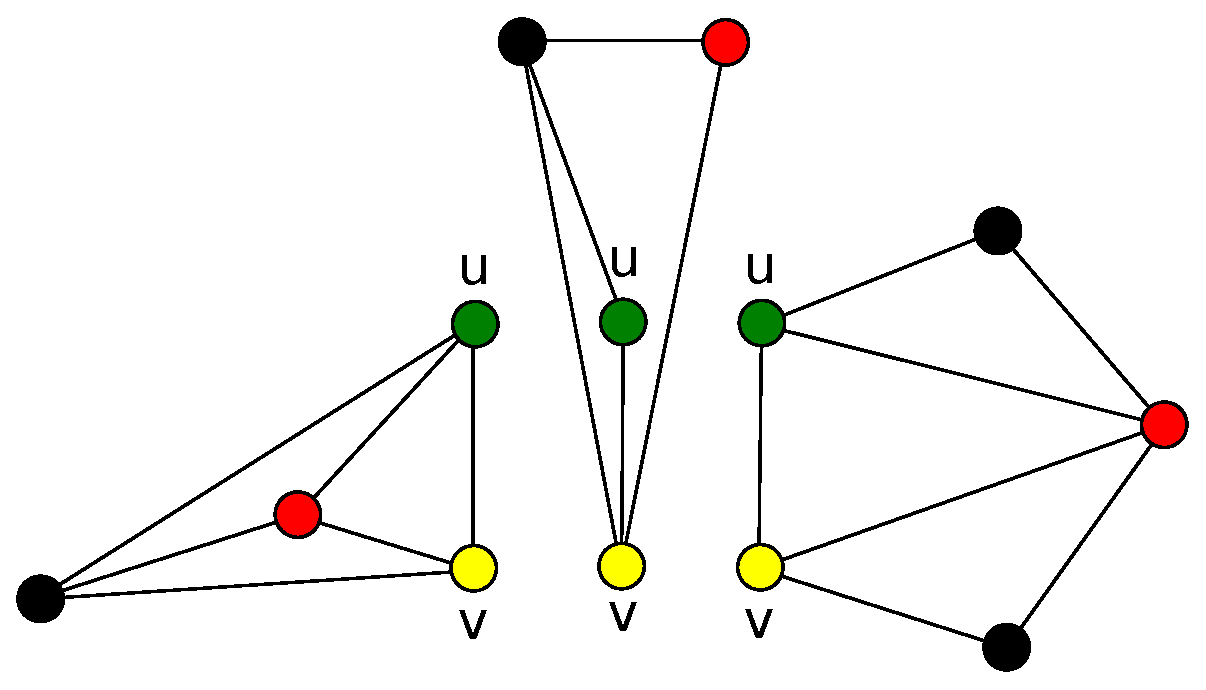
\includegraphics[scale=0.3]{s-comp-col.eps}           
    \end{figure}
}

\end{frame}


\begin{frame}{Teorema 8.2}{}

    \only<1>{
    \begin{alertblock}{Teorema}
           Em um grafo \textit{k-crítico}, nenhum corte por vértice é uma clique.
    \end{alertblock}
    }
    
    \only<2>{
    \begin{block}{Prova:}
        \begin{sloppypar}
        \justifying
        Por contradição. Seja $G$ um grafo $k$\textit{-crítico}, e suponha que $G$ possui um corte por vértice $S$ que é uma clique. 
        \vskip 0.3cm
        Denote as $S$\textit{-componentes} de $G$ por $G_1, G_2, \dots, G_n$. Uma vez que $G$ é $k$\textit{-crítico}, cada $G_i$ é $(k-1)$\textit{-colorível}. Além disso, como $S$ é uma clique, os vértices em $S$ precisam receber cores distintas em qualquer $(k-1)$\textit{-coloração} de $G_i$.
        
        \vskip 0.3cm
         Segue então, que existem $(k-1)$\textit{-colorações} de $G_1, G_2, \dots, G_n$ que concordam em $S$. Porém, essas colorações juntas produzem uma $(k-1)$-coloração de $G$, que é uma contradição, pois $G$ é \textit{k-crítico}.
        
        \hfill\(\square\)
        \end{sloppypar}
    \end{block}
    }
\end{frame}


\begin{frame}{Corolário 8.2}{}

    \begin{alertblock}{Corolário}
        Todo grafo crítico é um bloco. 
    \end{alertblock}
    \vskip 0.5cm
    \begin{block}{Prova:}
        \begin{sloppypar}
            \justifying
            Se $v$ é um vértice de corte, então \{$v$\} é um corte por vértice que também é uma clique. Portanto, segue do teorema $8.2$ que nenhum grafo crítico tem um vértice de corte.
            \hfill\(\square\)
        \end{sloppypar}
    \end{block}
        
\end{frame}


\begin{frame}{Consequência do Teorema 8.2}{}

    \vskip 0.2cm
    \begin{outline}    
        \1[] \justifying Uma consequência do teorema 8.2 é que se um grafo $G$ \textit{k-crítico} tem  um 2-\textit{corte por vértice} $\{u, v\}$, então $u$ e $v$ \textbf{não} podem ser adjacentes. 
        \vskip 0.4cm
        \2 \begin{sloppypar} \justifying Veremos que um $\{u, v\}$\textit{-componente} $G_i$ de $G$ é do \textbf{tipo 1}, se toda \textit{(k-1)-coloração} de $G_i$ atribui as mesmas cores para $u$ e $v$. E é do \textbf{tipo 2}, se toda \textit{(k-1)-coloração} de $G_i$ atribui cores diferentes para $u$ e $v$. \end{sloppypar}    

    \end{outline}
    
    %Inserir Figura 8.4
    \begin{figure}
      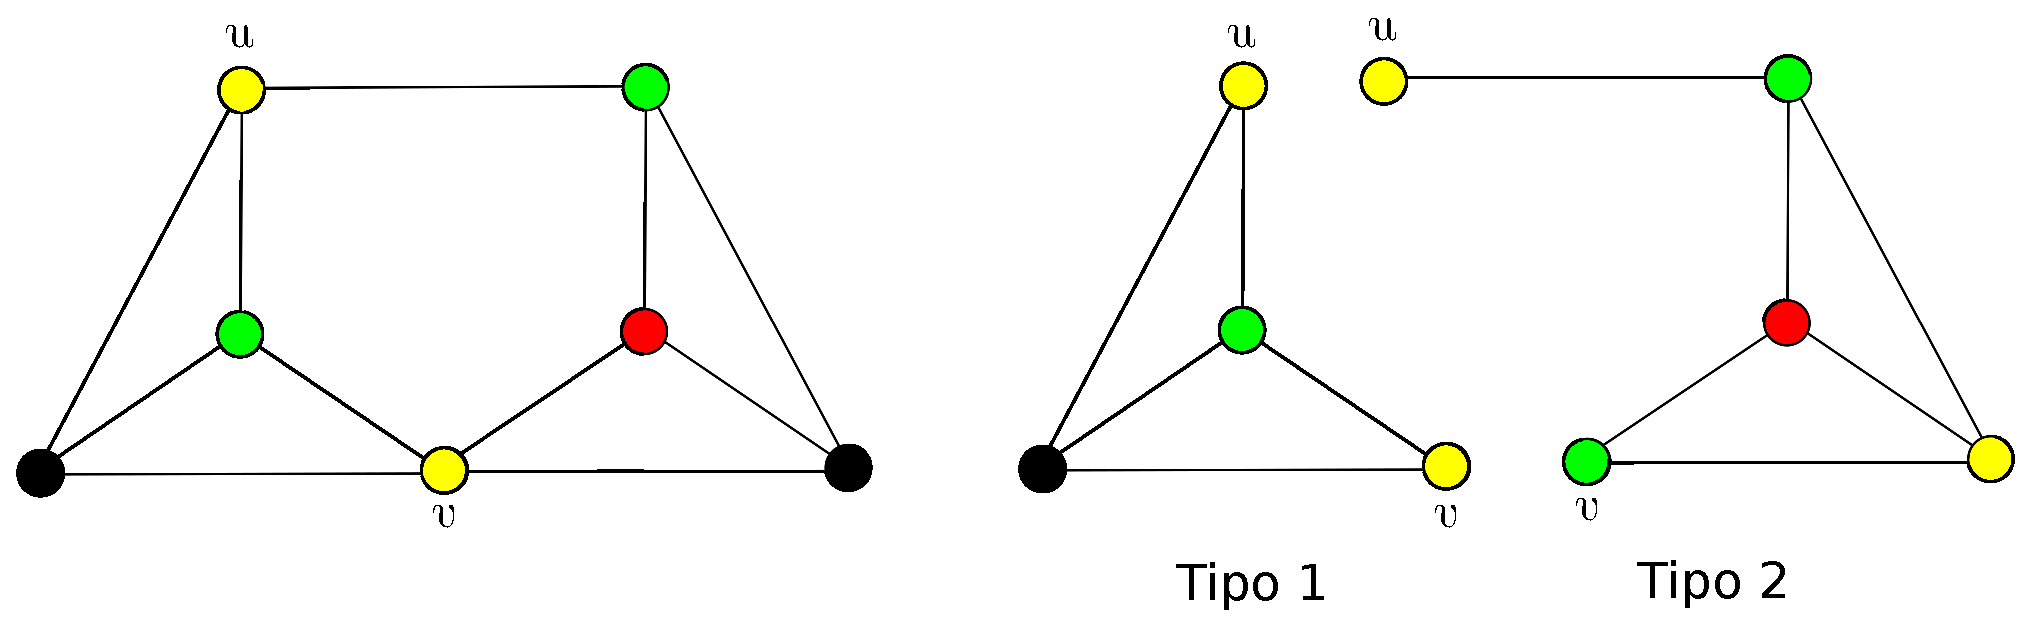
\includegraphics[scale=0.3]{tipos.eps}      
      \caption{}      
    \end{figure}  

\end{frame}


\section{Teorema 8.3}
\begin{frame}{Teorema 8.3}{(Dirac, 1953)}

   \only<1>{ \begin{alertblock}{Teorema 8.3}
        Seja $G$ um grafo \textit{k-crítico} com um \textit{2-corte por vértices} $\{u, v\}$. Então:
        \vskip 0.05cm
        \begin{outline}
            \1[1.] $G = G_1 \cup G_2$, onde $G_i$ é um $\{u, v\}$\textit{-componente} do tipo tipo $i$ ($i=\{1, 2\}$) e,
            \vskip 0.2cm
            \1[2.] Ambos $G_1 + uv$ e $G_2 \cdot uv$ são \textit{k-crítico} (onde $G_2 \cdot uv$ denota o grafo obtido a partir da contração dos vértices $u$ e $v$).
        \end{outline}
    \end{alertblock}
    
    % Colocar uma figura aqui
    \begin{figure}
      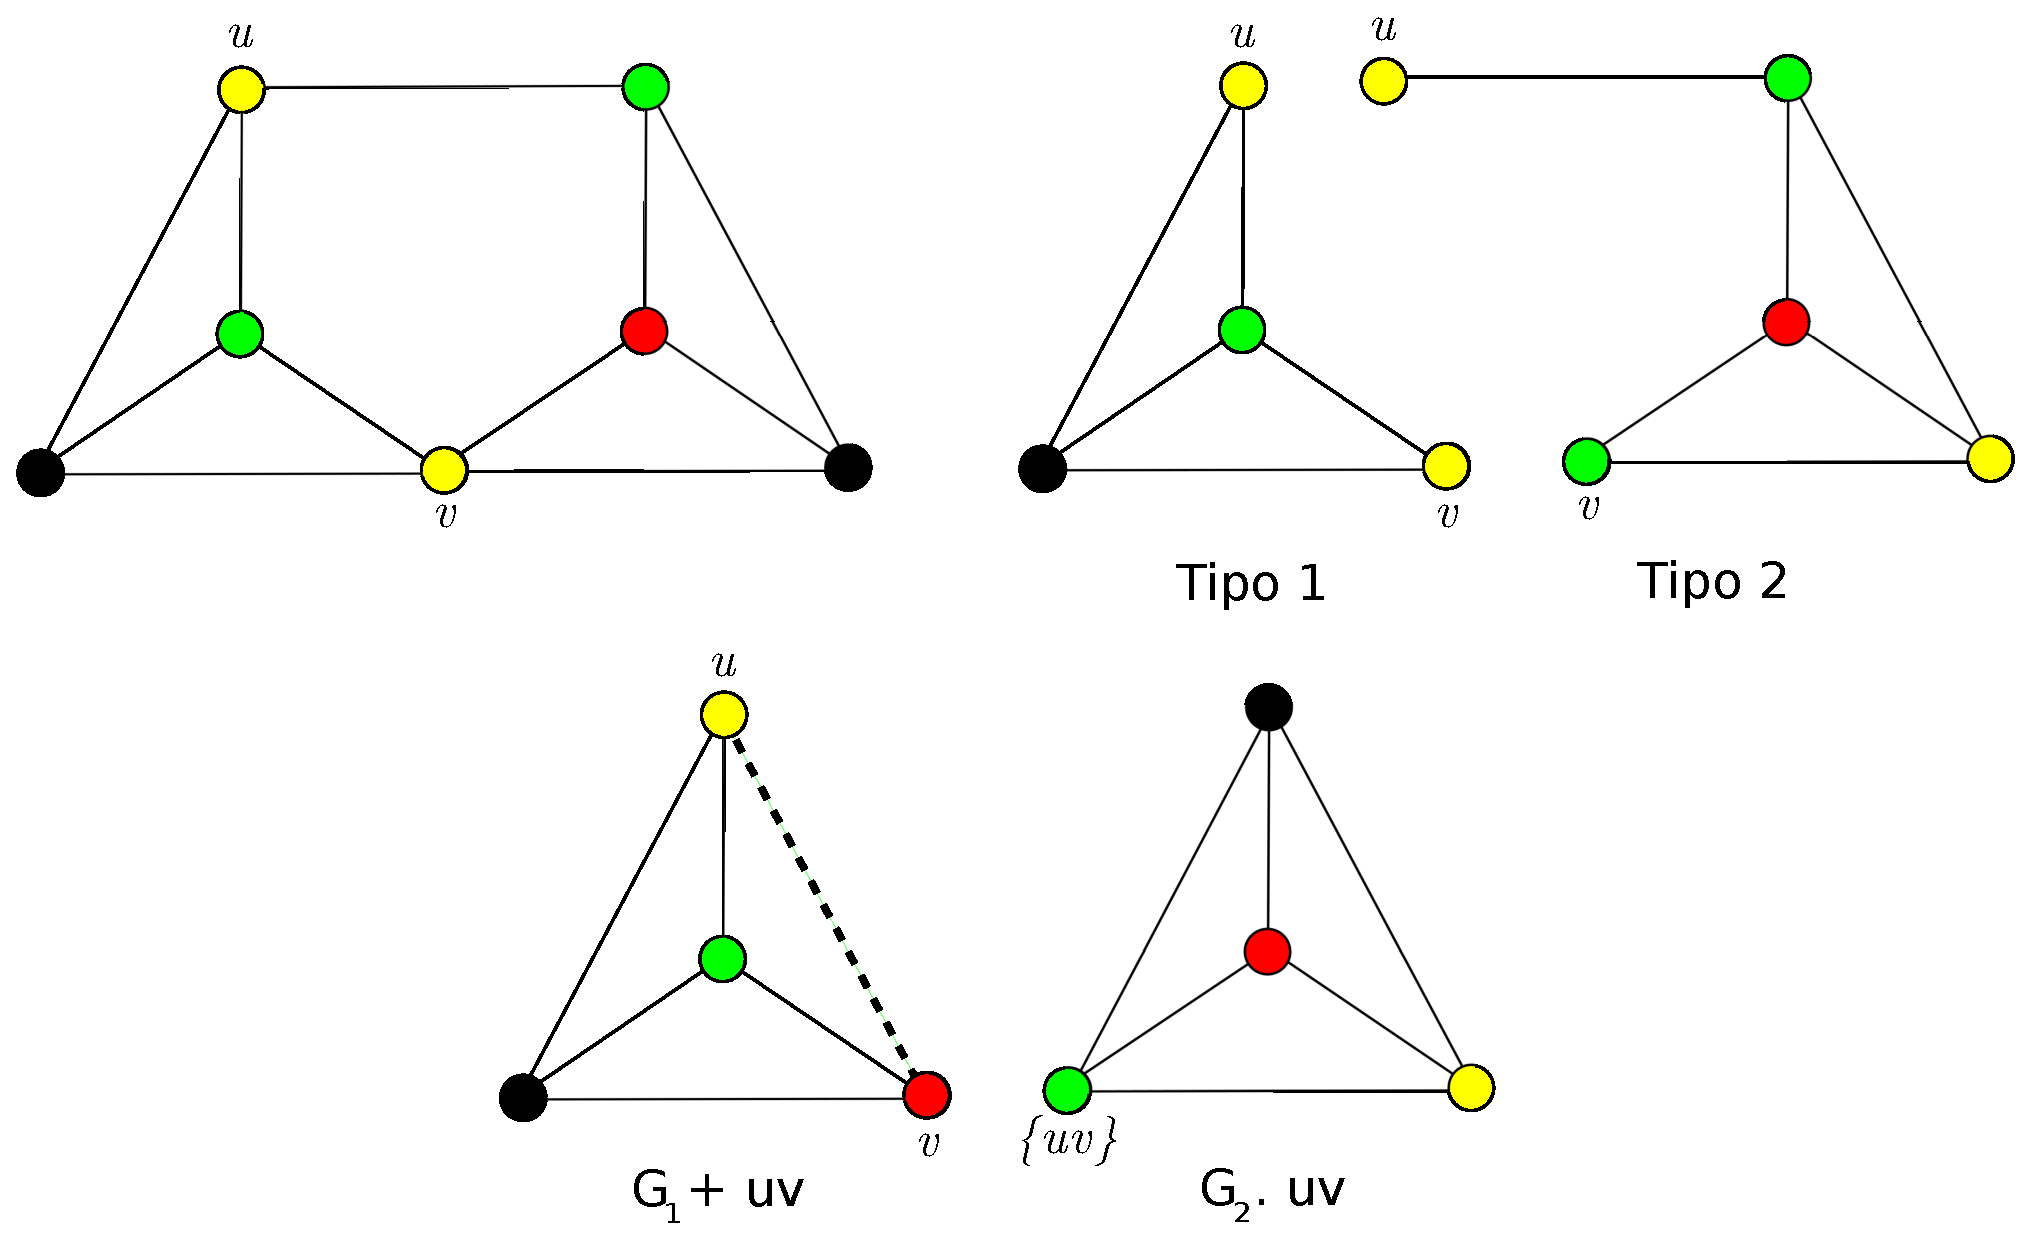
\includegraphics[scale=0.2]{tipos2.eps}      
      \caption{}      
    \end{figure}  
    
    }
    
    \only<2>{
    
    \begin{block}{Prova:}
    \begin{sloppypar}
      1. \justifying Como $G$ é crítico, cada $\{u, v\}$\textit{-componente} de $G$ é \textit{(k-1)-colorível}. Portanto, não pode existir \textit{(k-1)-colorações} em todos estes $\{u, v\}$\textit{-componentes} que \textit{concordam} em $\{u, v\}$, já que tais colorações iriam juntos produzir uma \textit{(k-1)-coloração} em G. 
      
      \vskip 0.30cm
      Logo, há dois $\{u, v\}$\textit{-componentes} $G_1$ e $G_2$ tal que nenhuma \textit{(k-1)-coloração} de $G_1$ concorda com alguma \textit{(k-1)-coloração} de $G_2$.
      
    \vskip 0.3cm
    Claramente um, digamos $G_1$, deve ser do tipo 1 e outro, $G2$, do tipo 2. Como $G1$ e $G2$ são de tipos diferentes, o subgrafo $G_1 \cup G_2$ de $G$ \textbf{não é} \textit{(k-1)-colorível}. Assim, como $G$ é crítico, temos que ter $G = G_1 \cup G_2$.
    
    \end{sloppypar}
    \end{block}
    }
      
        

    \only<3>{
    
    \begin{block}{Prova:}
        \begin{sloppypar}
          2. Faça $H_1 = G_1 + uv$. Como $G_1$ é do tipo 1, $H_1$ é \textit{k-cromático}. Iremos provar que $H_1$ é crítico, mostrando que para cada aresta \textbf{\textit{e}} de $H_1$, $H_1 - e$ é \textit{(k-1)-colorível}. 
          \vskip 0.3cm
           Isso claramente é  verdade se $e = uv$, pois $H_1-e = G_1$.
          \vskip 0.30cm
          \justifying Seja $e$ outra aresta de $H_1$. Em Qualquer \textit{(k-1)-coloração} de $G-e$, os vértices $u$ e $v$ devem receber cores diferentes, já que $G_2$ é um subgrafo de $G-e$. A restrição de tal coloração nos vértices de $G_1$ é uma \textit{(k-1)-coloração} de $H_1  - e$. Portanto, $G_1 + uv$ é crítico. Um argumento análogo mostra que $G_2 \cdot uv$ é \textit{k-crítico} \hfill\(\square\)
          
        \end{sloppypar}
    \end{block}
    }
      
  
    
    
  
    
\end{frame}



\begin{frame}{Corolário 8.3}

    \begin{alertblock}{Corolário}
        Seja $G$ um grafo $k$\textit{-crítico} com um \textit{2-corte por vértice} $\{u,v\}$. Então: 
        \begin{equation}
            d(u) + d(v) \geq 3k - 5
        \end{equation}
    \end{alertblock}
    \vskip 0.3cm
    \begin{block}{Prova:}
        \begin{sloppypar}
            \justifying
            Seja $G_1$ o $\{u,v\}$\textit{-componente} do tipo 1 e $G_2$ o $\{u,v\}$\textit{-componente} do tipo 2. Faça $H_1 = G_1 + uv$ e $H_2 = G_2 \cdot uv$. Pelos teoremas 8.3 e 8.1, temos:
            \vskip 0.05cm
           
            \begin{equation*}
                d_{H_1}(u) + d_{H_1}(v) \geq 2k - 2\ \ \text{e} \ \ d_{H_2}(w) \geq k - 1
            \end{equation*}
            \textit{onde $w$ é o novo vértice obtido por identificar (contrair) $u$ e $v$.}
            \vskip 0.12cm
            Segue que:
            \begin{equation*}
                d_{G_1}(u) + d_{G_1}(v) \geq 2k - 4\ \ \text{e}\ \ 
                d_{G_2}(u) + d_{G_2}(v) \geq k-1
            \end{equation*}
            Essas duas inequações produzem (8.1)
            \hfill\(\square\)
        \end{sloppypar}
    \end{block}
        
\end{frame}

\begin{frame}{Teorema de Brooks}{Teorema 8.4}

    \begin{itemize}
          \item O teorema de Vizing ($\chi' = \Delta$ ou $\chi' = \Delta+1$) é um resultado consideravelmente mais forte do que o \textit{upper bound} dado no corolário 8.1.2 ($\chi \leq \Delta+1$).
    \end{itemize}
    
    
    \begin{alertblock}{Teorema 8.4}
       Se $G$ é um grafo simples conexo e não é um ciclo ímpar e também não é um grafo completo, então $\chi \leq \Delta$
       
    \end{alertblock}
    \vskip 0.2cm
    \begin{block}{Prova:}
        \begin{sloppypar}
            \justifying
            Seja $G$ um grafo $k$\textit{-cromático} que satisfaz a hipótese do teorema. Sem perda de generalidade, podemos assumir que $G$ é $k$\textit{-crítico}. Pelo corolário 8.2, $G$ é um bloco. Além disso, uma vez que grafos $1$\textit{-crítico} e $2$\textit{-crítico} são completos e grafos $3$\textit{-crítico} são ciclos ímpares, temos que $k \geq 4$. 
            
        \end{sloppypar}
    \end{block}
        
\end{frame}


\begin{frame}{Teorema de Brooks}{Teorema 8.4}

    
    \begin{block}{Prova (cont.):}
        \begin{sloppypar}
            \justifying
            Se $G$ tem um \textit{2-corte por vértice} $\{u,v\}$, usando o corolário 8.3, temos que:
            \begin{equation*}
                2\Delta \geq d(u) + d(v) \geq 3k - 5 \geq 2k - 1
            \end{equation*}
            Isso implica que $\chi = k \leq \Delta$, uma vez que $2\Delta$ é par.
        \end{sloppypar}
    \end{block}
        
\end{frame}

\begin{frame}{Teorema de Brooks}{Teorema 8.4}

    
    \begin{block}{Prova (cont.):}
        \begin{sloppypar}
            \justifying
            Assuma que $G$ é \textit{3-conexo}. Uma vez que $G$ não é completo, existem três vértices $u,v$ e $w$ em $G$ tal que $uv, vw \in E$ e $uw \notin E$. 
            \vskip 0.3cm
            Faça $u = v_1$ e $w = v_2$ e seja $v_3, v_4, \dots, v_v=v$ qualquer ordem dos vértices de $G-\{u,w\}$ tal que cada $v_i$ é adjacente a algum $v_j$ com $j > i$. (Isso pode ser alcançado por arranjar os vértices em ordem não crescente de sua distância de $v$).
            \vskip 0.3cm
            Podemos agora descrever uma $\Delta$\textit{-coloração } de $G$: 
            \vskip 0.1cm
            
            \begin{outline}
            \1[1.] atribua \textbf{cor 1} para $v_1=u$ e $v2=w$;
            \1[2.] então, sucessivamente, colore $v_3,v_4,\dots,v_v$ com a primeira cor disponível na lista $1,2,\dots,\Delta$.                
            \end{outline}          
            
        \end{sloppypar}
    \end{block}
        
\end{frame}

\begin{frame}{Teorema de Brooks}{Teorema 8.4}

    \begin{figure}
      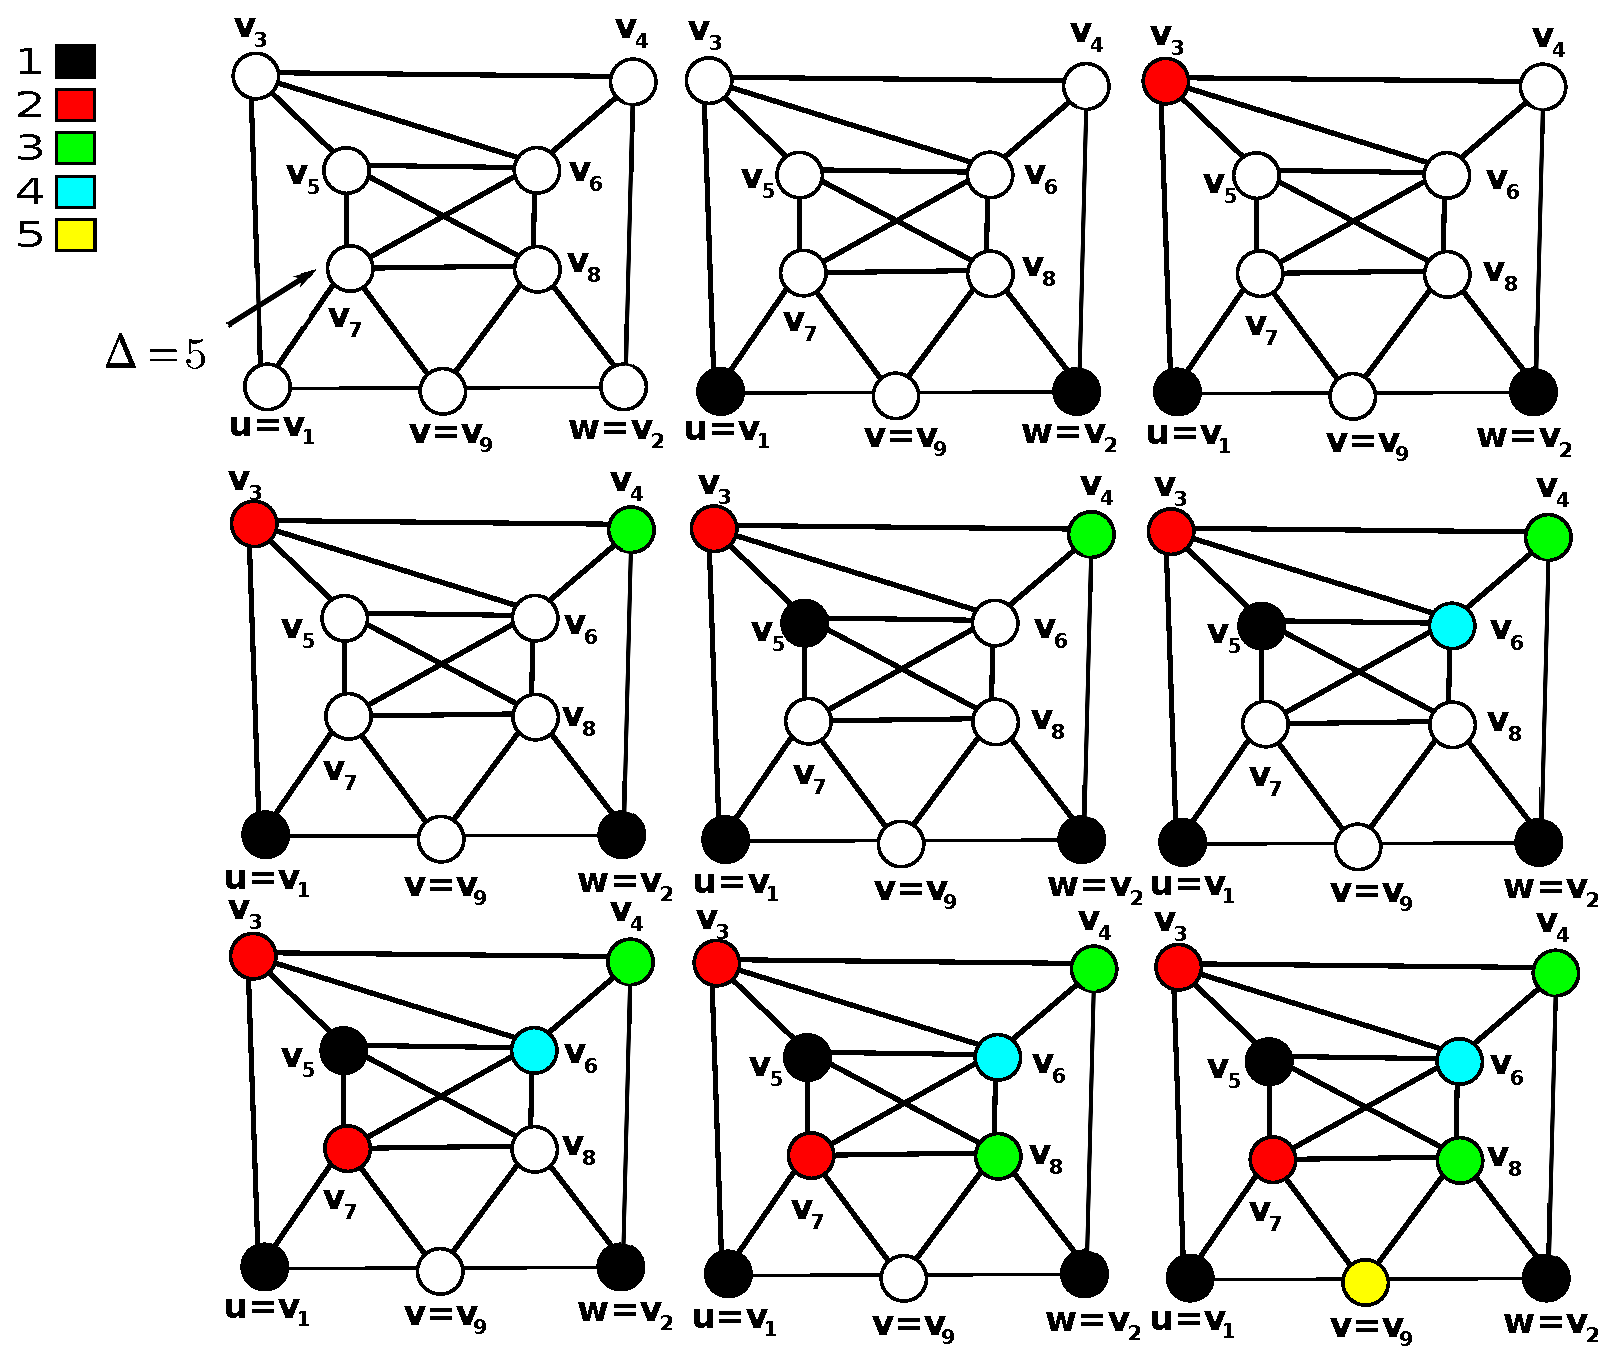
\includegraphics[scale=0.35]{delta-coloring.eps}           
    \end{figure}
        
\end{frame}

\begin{frame}{Teorema de Brooks}{Teorema 8.4}

    
    \begin{block}{Prova (cont.):}
        \begin{sloppypar}
            \justifying
            Pela construção da sequência $v_1,v_2,\dots,v_v$, cada vértice $v_i$, $1 \leq i \leq v-1$, é adjacente a algum vértice $v_j$ com $j > i$, e a no máximo $\Delta-1$ vértices $v_i$ com $j<i$.
            
            \vskip 0.3cm
            Segue que, quando $v_i$ for colorido, $v_i$ é adjacente a no máximo $\Delta - 1$ cores, e portanto uma das cores $1,2,\dots,\Delta$ estará disponível.
            \vskip 0.3cm
            Finalmente, uma vez que $v_v$ é adjacente a dois vértices de cor $1$ ($v_1$ e $v_2$), $v_v$ é adjacente a no máximo $\Delta-2$ outras cores e pode receber uma das cores $2,3,\dots,\Delta$.
            
            \hfill\(\square\) 
            
        \end{sloppypar}
    \end{block}
        
\end{frame}


        


\begin{frame}{Conjectura de Hajó}{}
    
    \begin{block}{Conjecture de Hajó}
        Se $G$ é \textit{k-cromático}, então $G$ contém uma subdivisão de $K_k$.        
    \end{block}
    \vskip 0.2cm
    
\only<1>{
    Uma subdivisão de um grafo $G$ é um grafo que pode ser obtido a partir de $G$, por uma sequência de divisões de arestas.
    
     \begin{figure}
      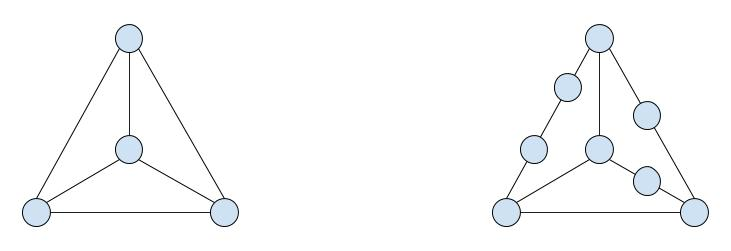
\includegraphics[scale=0.3]{k4_sub.jpg}      
      \caption{Subdivisões de um $K_4$.}      
    \end{figure}
        
    
        \alert{Note que essa condição não é suficiente; por exemplo, um \textit{4-ciclo} é uma subdivisão de um $k_3$, mas não é \textit{3-cromático}}
        
        
    }
    \vskip 0.3cm
    \only<2>{
      Para $k = 1$ e $k = 2$ a validade da conjectura de Hajós é óbvia. A conjectura também é facilmente verificada para $k = 3$, pois um grafo \textit{3-cromático} necessariamente contém um ciclo ímpar, e todo ciclo ímpar é subdivisão do $k_3$. Dirac (1952) provou o caso de $k = 4$.
    
    }      
        
        
\end{frame}


\begin{frame}{Teorema 8.5}

\only<1>{

\begin{alertblock}{Teorema}
Se $G$ é \textit{4-cromático}, então $G$ contém uma subdivisão do $K_4$.
\end{alertblock}
    
  
    
    \begin{block}{Prova}
        \begin{sloppypar}
            \justifying
            Seja $G$ um grafo \textit{4-cromático}. Note que se algum subgrafo de $G$ contiver uma subdivisão do $K_4$, então $G$ também terá.
            
            \vskip 0.3cm
            Sem perda de generalidade, podemos assumir que $G$ é crítico, e portanto que $G$ é um bloco com $\delta \geq 3$ (teorema $8.1$). Se $n = 4$, então $G$ é $K_4$ (caso trivial).
            
            \vskip 0.5cm
            
            Por indução em $n$, assuma que o teorema é válido para todo grafo \textit{4-cromático} com menos de $n$ vértices, e seja  $n(G) = n > 4$
           
           
        \end{sloppypar}
    \end{block}
    }
    
    \only<2>{
    \begin{block}{Prova}
        \begin{sloppypar}
            \justifying
            Primeiro, suponha que $G$ tem um \textit{2-corte por vértice} $\{u, v\}$. Pelo teorema 8.3, $G$ tem dois $\{u,v\}$\textit{-componentes} $G_1$ e $G_2$, onde $G_1 + uv$ é \textit{4-crítico}.          
            
            \vskip 0.3cm 
            Como $n(G_1 + uv) < n(G)$, podemos aplicar a hipótese de indução e deduzir que $G_1 + uv$ contém uma subdivisão do $K_4$. 
            
            \vskip 0.3cm
            Segue que, como $P$ é um $(u,v)$\textit{-caminho} em $G_2$,  então $G_1 \cup P$ contém uma subdivisão do $K_4$. Como $G_1 \cup P \subseteq G$, então $G$ também contém uma subdivisão do $K_4$
           
            
        \end{sloppypar}
    \end{block}
    
    
    }
    
    
    \only<3>{
    \begin{block}{Prova}
        \begin{sloppypar}
            \justifying
            Agora, suponha que $G$ é \textit{3-conexo}. Como $\delta \geq 3$, $G$ tem um ciclo $C$ de tamanho $\geq 4$.
            \vskip 0.3cm
            Sejam $u$ e $v$ vértices não consecutivas em $C$. Como $G-\{u, v\}$ é conexo, existe um caminho $P$ em $G-\{u, v\}$ conectando as duas componentes de $C-\{u,v\}$; podemos assumir que a origem $x$ e o término $y$ são os únicos vértices de $P$ em $C$. De forma similar, há um caminho $Q$ em $G-\{x, y\}$. % adicionar Figura 8.6
            \vskip 0.5cm
            
            Se $P$ e $Q$ não têm nenhum vértice em comum, então $C \cup P \cup Q$ é uma subdivisão do $K_4$. Caso contrário, seja $w$ o primeiro vértice de $P$ em $Q$, e denote por $P'$ a $(x,w)$\textit{-seção} de $P$. Então  $C \cup P' \cup Q$ é uma subdivisão do $K_4$. Logo, em ambos os casos, $G$ contém uma subdivisão do $K_4$.
           
            \hfill\(\square\)
        \end{sloppypar}
    \end{block}
    
    
    }
    
    \only<4>{
    \begin{center}
        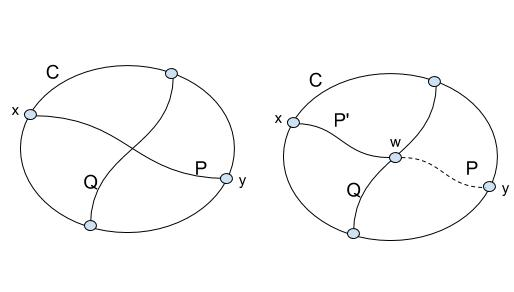
\includegraphics[scale=0.6]{85.jpg}  
    \end{center}
    
    }

        
\end{frame}


\begin{frame}{Teorema}{8.7}

\only<1-2>{
\begin{alertblock}{Teorema 8.7}
Para qualquer inteiro $k$ positivo, existe um grafo \textit{k-cromático} que não contém triângulos.
\end{alertblock}
}

\only<2>{
\begin{block}{Prova:}
\justifying
Para $k = 1$ e $k = 2$, os grafos $K_1$ e $K_2$ apresentam a propriedade requerida. Prosseguimos por indução em $k$.


\vskip 0.3cm
Suponha que tenhamos construído um grafo $G_k$ sem triângulo com um número cromático $k \geq 2$. Sejam $v_1, v_2, \ldots, v_n$ os vértices de $G_k$. Forme um novo grafo $G_{k+1}$ a partir de $G_k$ da seguinte forma:
\vskip 0.2cm

\begin{outline}
    \1[1.] Adicione $n+1$ novos vértices  $u_1, u_2, \ldots, u_n, v$,
    \vskip 0.1cm
    \1[2.] e então, para $1 \leq i \leq n$, una $u_i$ aos vizinhos de $v_i$ e a $v$.
\end{outline}


\end{block}


% \begin{figure}
%   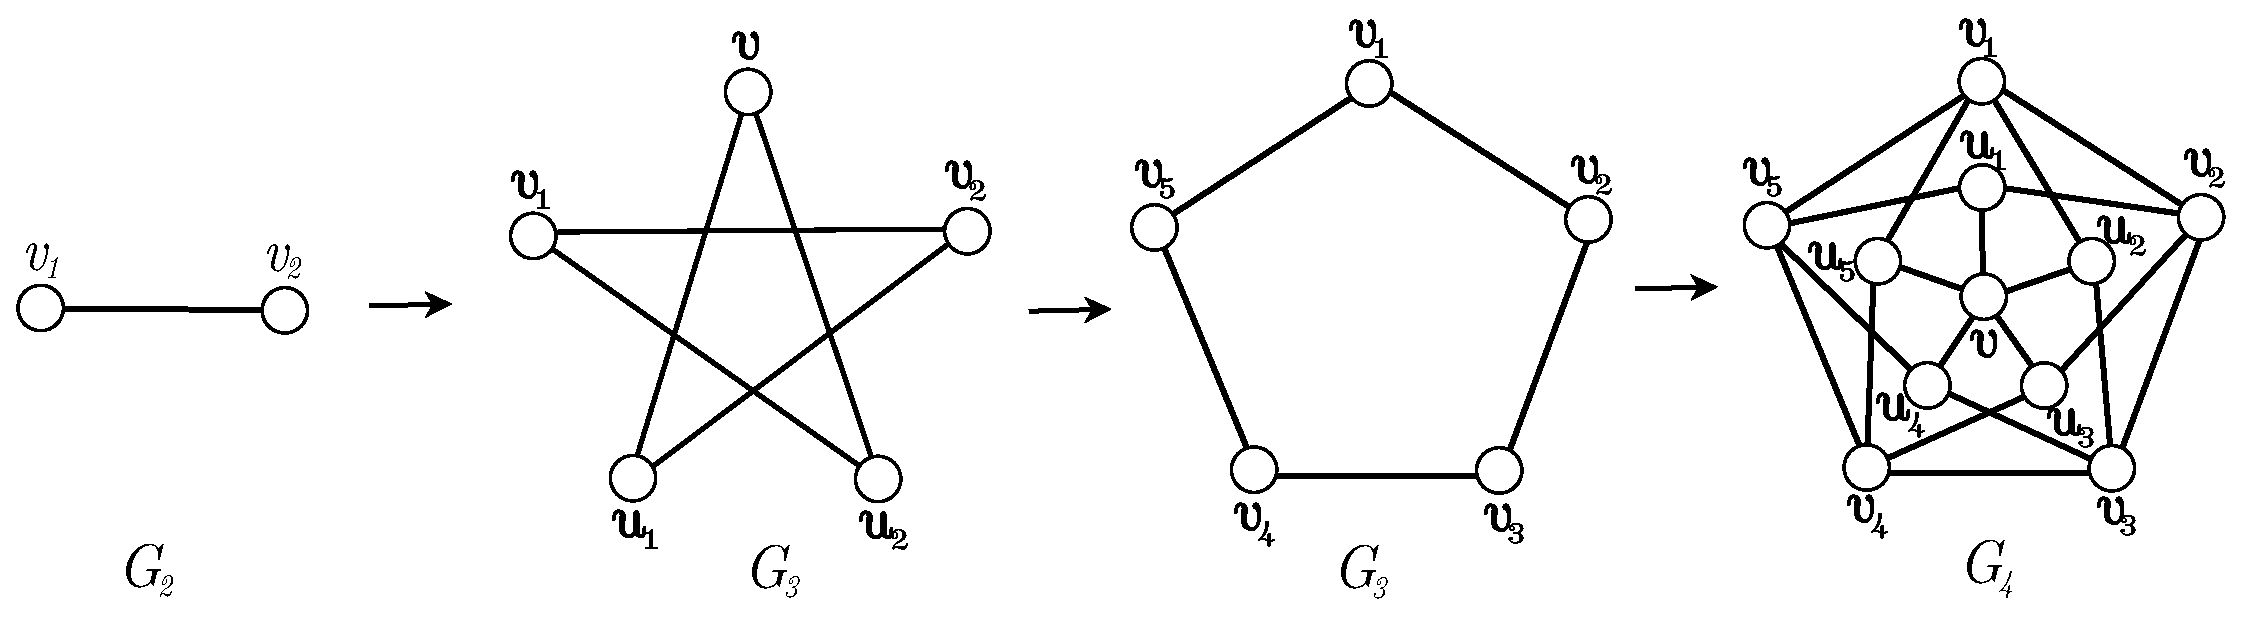
\includegraphics[scale=0.3]{mycielski.eps}      
%   %\caption{Subdivisões de um $K_4$.}      
% \end{figure}


}

\end{frame}


% Figuras
\begin{frame}{Teorema}{8.7}

\begin{center}
\only<1>{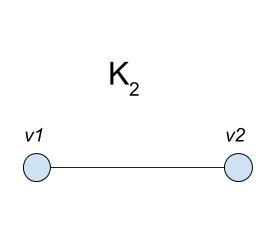
\includegraphics[scale=0.4]{k2.jpg}}
            
\only<2>{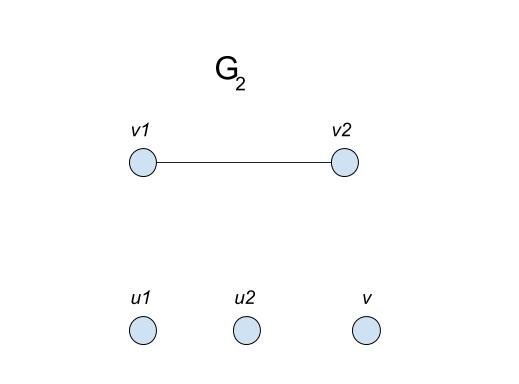
\includegraphics[scale=0.4]{87_1.jpg}}

\only<3>{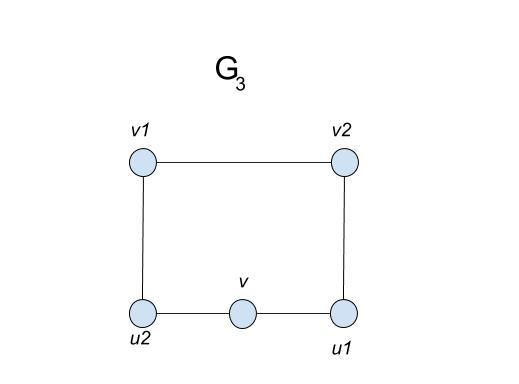
\includegraphics[scale=0.4]{87_2.jpg}}
\end{center}


\end{frame}


            




\begin{frame}{Teorema}{8.7}

\only<1>{

    \begin{block}{Prova:}
    
        \justifying
        Claramente, o grafo $G_{k+1}$ não tem triângulos. Pois, como $\{u_1, u_2, \ldots, u_n\}$ é um conjunto independente em $G_{k+1}$, nenhum triângulo pode conter mais que um $u_i$; e se $u_{i}v_{j}v_{k}u_{i}$ eram um triângulo em $G_{k+1}$, então  $v_{i}v_{j}v_{k}v_{i}$ seria um triângulo em $G_k$, contrariando o pressuposto.
        
        \vskip 0.5cm
        
        Mostraremos agora que $G_{k+1}$ é \textit{(k+1)-cromático}.
        
        
        \vskip 0.5cm 
        \textit{Note que $G_{k+1}$ é certamente \textit{(k+1)-colorível}, já que qualquer coloração de $G_k$ pode ser estendida para uma \textit{(k+1)-coloração} em $G_{k+1}$ colorindo $u_i$ do mesmo modo que $v_i$, $1 \leq i \leq n$, e então atribuindo uma nova cor para $v$.}
        
        \vskip 0.2cm
        
        Portanto, resta mostrar que $G_{k+1}$ \textbf{não} é \textit{k-colorível}.
    
    
    \end{block}

}


\only<2>{
    \begin{block}{Prova (cont):}
        \justifying
        Se possível, considere uma \textit{k-coloração} de $G_{k+1}$ no qual, sem perda de generalidade, $v$ é atribuído a cor $k$. Claramente, nenhum $u_i$ pode também ter a cor $k$. Agora, recolora cada vértice $v_i$, cuja cor é $k$, com a cor atribuída a $u_i$.
        
        \vskip 0.5cm
        
        Isso resulta em uma \textit{(k-1)-coloração} do grafo \textit{k-cromático}  $G_k$. Portanto, $G_{k+1}$ é também \textit{(k+1)-cromático}. O teorema segue pelo princípio da indução.
        
         \hfill\(\square\)
        
    
    \end{block}
}

        
\end{frame}


\begin{frame}
    \begin{center}
        Dúvidas?
    \end{center}
    
     \vskip 0.5cm
        %  Favor Manter os créditos dos autores%
        Todo os arquivos desta apresentação foram disponibilizados inicialmente em: \url{https://github.com/luanteylo/coloracao_vertices}
\end{frame}




\end{document}
